\documentclass[tikz,border=2pt]{standalone}
\usepackage[T1]{fontenc}
\usepackage[utf8]{inputenc}
\usepackage{lmodern}
\usepackage{pgfplots}
\pgfplotsset{compat=1.17}
\begin{document}
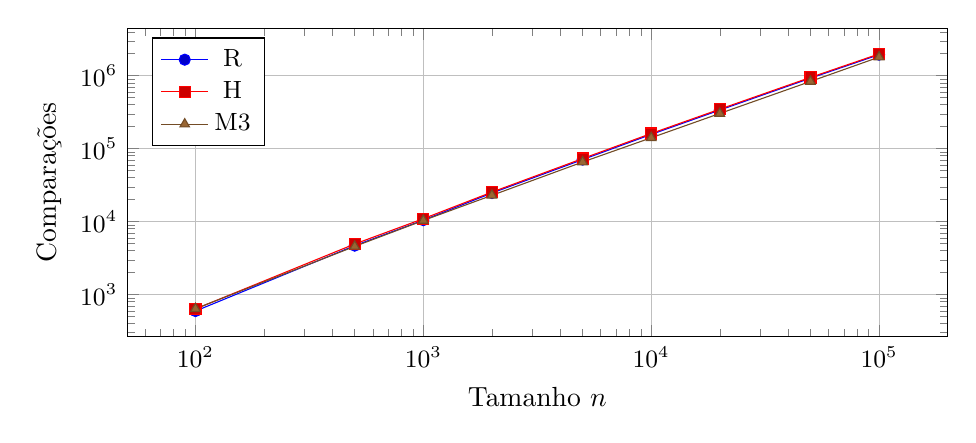
\begin{tikzpicture}
\begin{axis}[width=12cm,height=5.5cm,xmode=log,ymode=log,xlabel={Tamanho $n$},ylabel={Comparações},grid=major,legend pos=north west,legend style={font=\small},tick label style={font=\small}]
\addplot+[mark=*] coordinates {(100,595) (500,4690) (1000,10481) (2000,24672) (5000,70861) (10000,156852) (20000,338200) (50000,924915) (100000,1943232)};
\addlegendentry{R}
\addplot+[mark=square*] coordinates {(100,636) (500,4940) (1000,10972) (2000,25389) (5000,73162) (10000,161474) (20000,347730) (50000,947781) (100000,1988771)};
\addlegendentry{H}
\addplot+[mark=triangle*] coordinates {(100,640) (500,4579) (1000,10373) (2000,22929) (5000,65611) (10000,141037) (20000,303752) (50000,834841) (100000,1799683)};
\addlegendentry{M3}
\end{axis}
\end{tikzpicture}
\end{document}
